\documentclass[12pt,a4paper]{ctexart}
\usepackage{amsmath}
\usepackage{amssymb}
\usepackage{graphicx}
\usepackage{float}
\usepackage{geometry}
\usepackage{subcaption}
\usepackage{booktabs}
\usepackage{array}
\usepackage{listings}
\usepackage{xcolor}
\usepackage{hyperref}
\geometry{a4paper, margin=1in}

\lstset{
    basicstyle=\ttfamily\footnotesize,
    keywordstyle=\color{blue},
    commentstyle=\color{gray},
    stringstyle=\color{red},
    numbers=left,
    numberstyle=\tiny\color{gray},
    stepnumber=1,
    numbersep=5pt,
    backgroundcolor=\color{white},
    showspaces=false,
    showstringspaces=false,
    showtabs=false,
    frame=single,
    tabsize=2,
    captionpos=b,
    breaklines=true,
    breakatwhitespace=false
}

% 设置中文字体为楷体
\setCJKmainfont{KaiTi} % 设置主字体为楷体
\setCJKsansfont{KaiTi} % 设置无衬线字体为楷体
\setCJKmonofont{KaiTi} % 设置等宽字体为楷体

\title{HW3：螺丝实例分割}
\author{李青雅 523030910004 电院2301}
\date{\today}

\begin{document}
\maketitle
\newpage
\tableofcontents % 生成目录
\newpage

\section{任务说明}
本次作业的目标是针对俯视角的 5 张螺丝图像实现相关算法，完成单个图像上的螺丝精确实例分割。要求能够准确地将每一个螺丝独立分割出来，避免漏分、误分割或不完整分割，并将分割结果通过叠加半透明彩色掩码进行可视化展示。

\section{方法介绍}

\subsection{算法选择}
本次作业采用**传统机器视觉方法**（基于 OpenCV）实现螺丝实例分割，未使用深度学习模型。传统方法在处理背景单一、对比度强烈的工业视觉检测任务时具有较高的执行效率和可解释性。

\subsection{核心处理流程}
算法的整体处理流程主要包含以下四个步骤：
\begin{enumerate}
    \item \textbf{图像预处理与降噪}：将彩色图像转换为灰度图，并应用 $5\times 5$ 的高斯滤波（Gaussian Blur）平滑图像，消除高频噪点。
    \item \textbf{自适应二值化}：由于各张测试图的背景光照与整体亮度有所不同，采用 Otsu 大津法计算自适应阈值，配合 \texttt{THRESH\_BINARY\_INV} 操作，将偏暗的螺丝和螺母作为前景（白色像素）提取出来。
    \item \textbf{形态学开运算}：使用 $3\times 3$ 的全1卷积核对二值图进行一次形态学开运算（Morphological Opening），切断极细小的毛刺并去除孤立的背景噪点。
    \item \textbf{实例提取与先验几何特征过滤}：
    \begin{itemize}
        \item \textbf{轮廓填充}：查找并填充所有前景连通域的内部空洞，获取每个物体的整体实心轮廓图（Filled Mask）。
        \item \textbf{面积过滤}：基于 \texttt{connectedComponentsWithStats} 获取每个连通域。首先剔除面积过小（$Area < 2000$）的微小斑点噪点。
        \item \textbf{实心率（Solid Ratio）过滤以剔除螺母}：因为测试集中混有大量内部具有大孔洞的螺母（干扰物），算法计算每个连通域的“原始像素面积”与“填充后面积”的比值（Solid Ratio）。螺母因为中空结构，实心率往往低于 0.75；而螺丝作为实心物体，实心率极高（接近 1）。因此设定阈值 $Ratio > 0.75$，成功剔除所有螺母，保留螺丝。
    \end{itemize}
    \item \textbf{掩码叠加与可视化着色}：对最终保留的每一个螺丝连通域进行重新编号（Instance ID），并为其随机分配不同的 RGB 颜色。使用 $Alpha=0.5$ 的权重将掩码叠加至原图，并在实例的外部轮廓上绘制红色边界线以增强显示效果。
\end{enumerate}

\section{结果展示}
以下展示了算法在 5 张测试图像上的实例分割可视化结果。左侧为原图，右侧为叠加了彩色半透明掩码及红色边缘线的分割结果图。

\begin{figure}[H]
    \centering
    \begin{subfigure}{0.48\textwidth}
        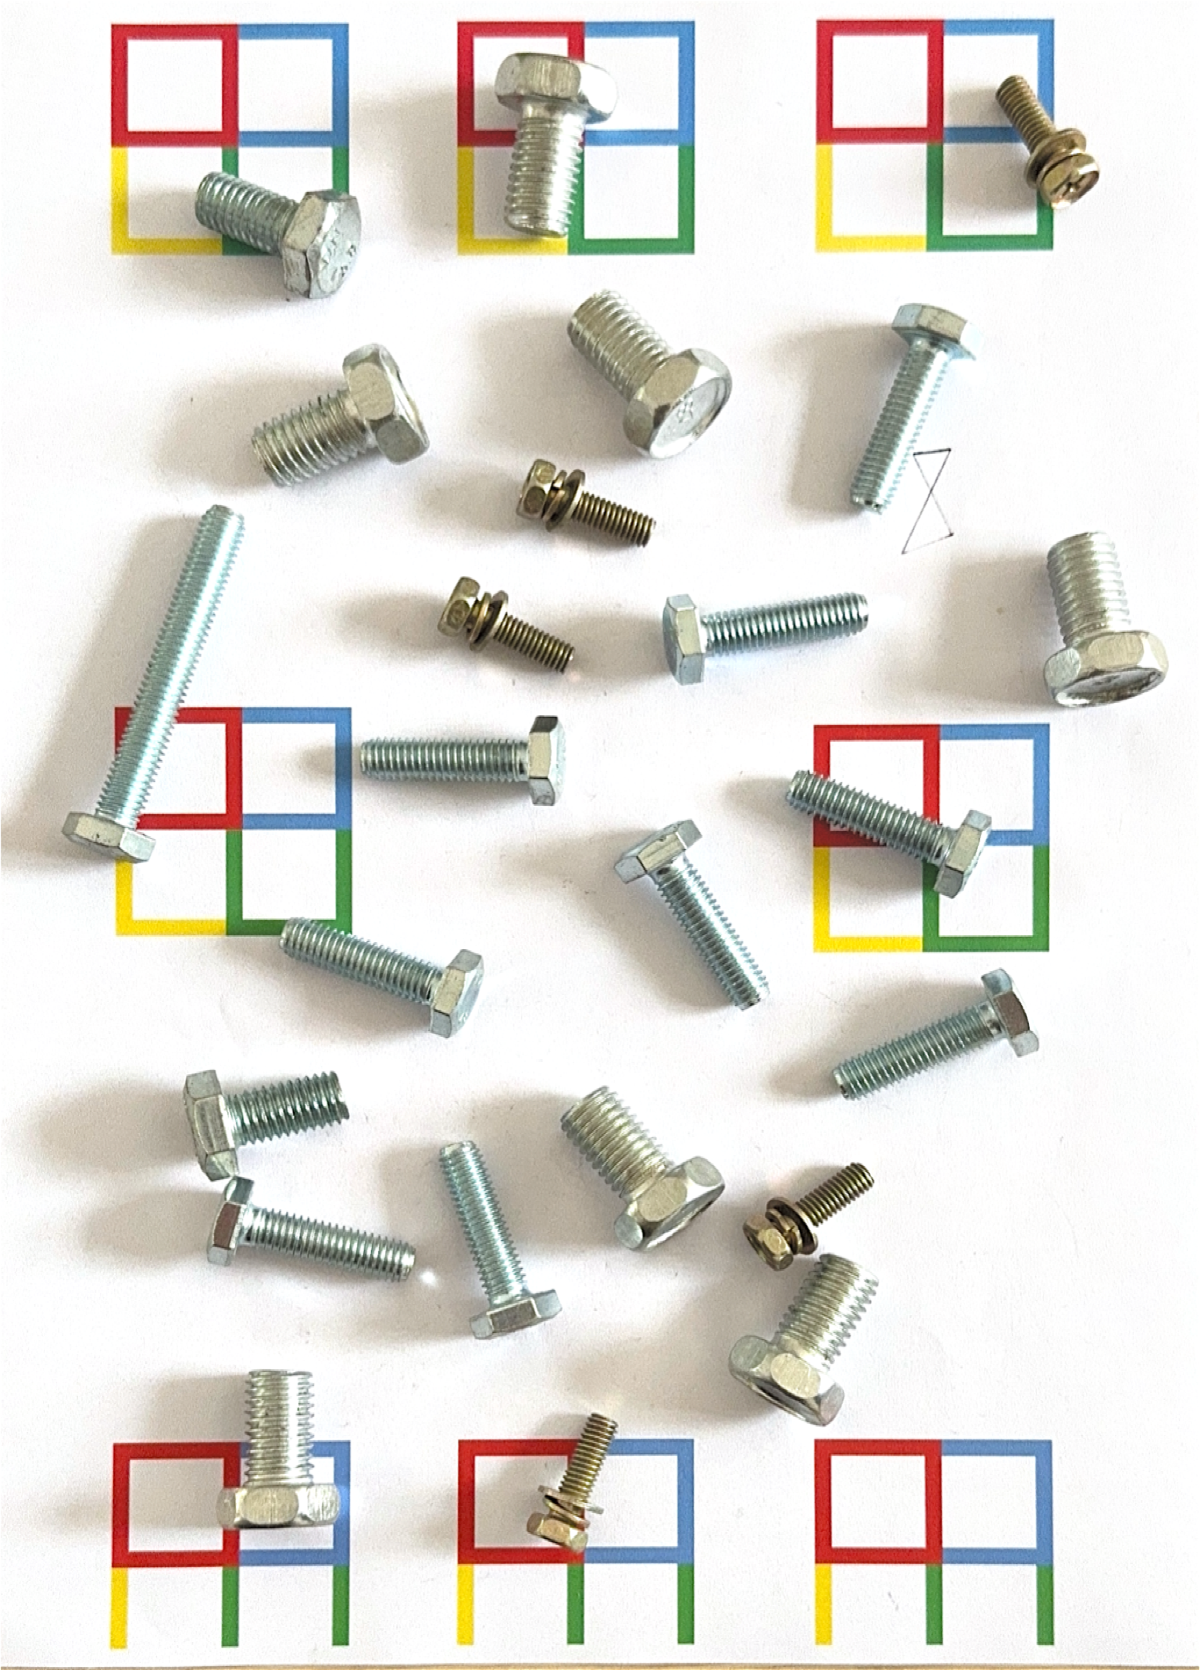
\includegraphics[width=\textwidth]{../data/01.png}
        \caption{01.png 原图}
    \end{subfigure}
    \begin{subfigure}{0.48\textwidth}
        
\includegraphics[width=\textwidth]{../output/01.png}
        \caption{01.png 分割结果 (共14个螺丝)}
    \end{subfigure}
\end{figure}

\begin{figure}[H]
    \centering
    \begin{subfigure}{0.48\textwidth}
        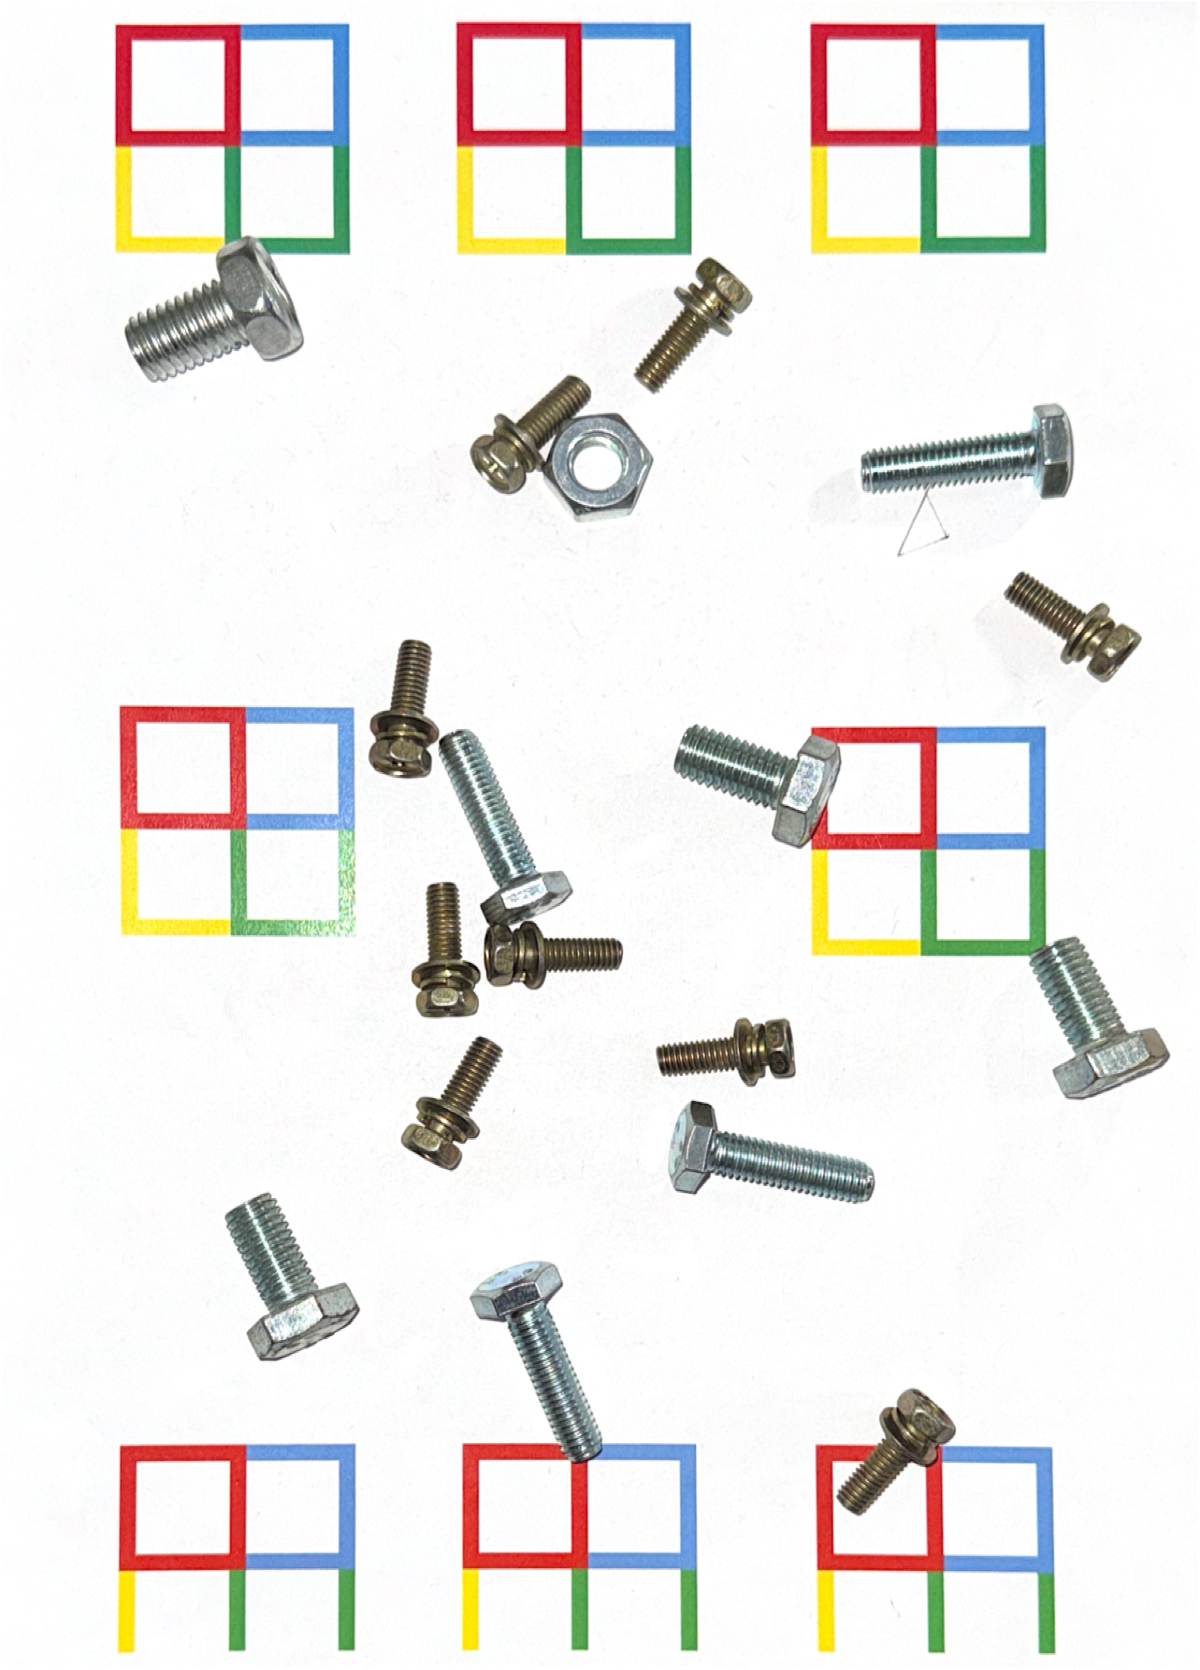
\includegraphics[width=\textwidth]{../data/04.png}
        \caption{04.png 原图}
    \end{subfigure}
    \begin{subfigure}{0.48\textwidth}
        
\includegraphics[width=\textwidth]{../output/04.png}
        \caption{04.png 分割结果 (共10个螺丝)}
    \end{subfigure}
\end{figure}

\begin{figure}[H]
    \centering
    \begin{subfigure}{0.48\textwidth}
        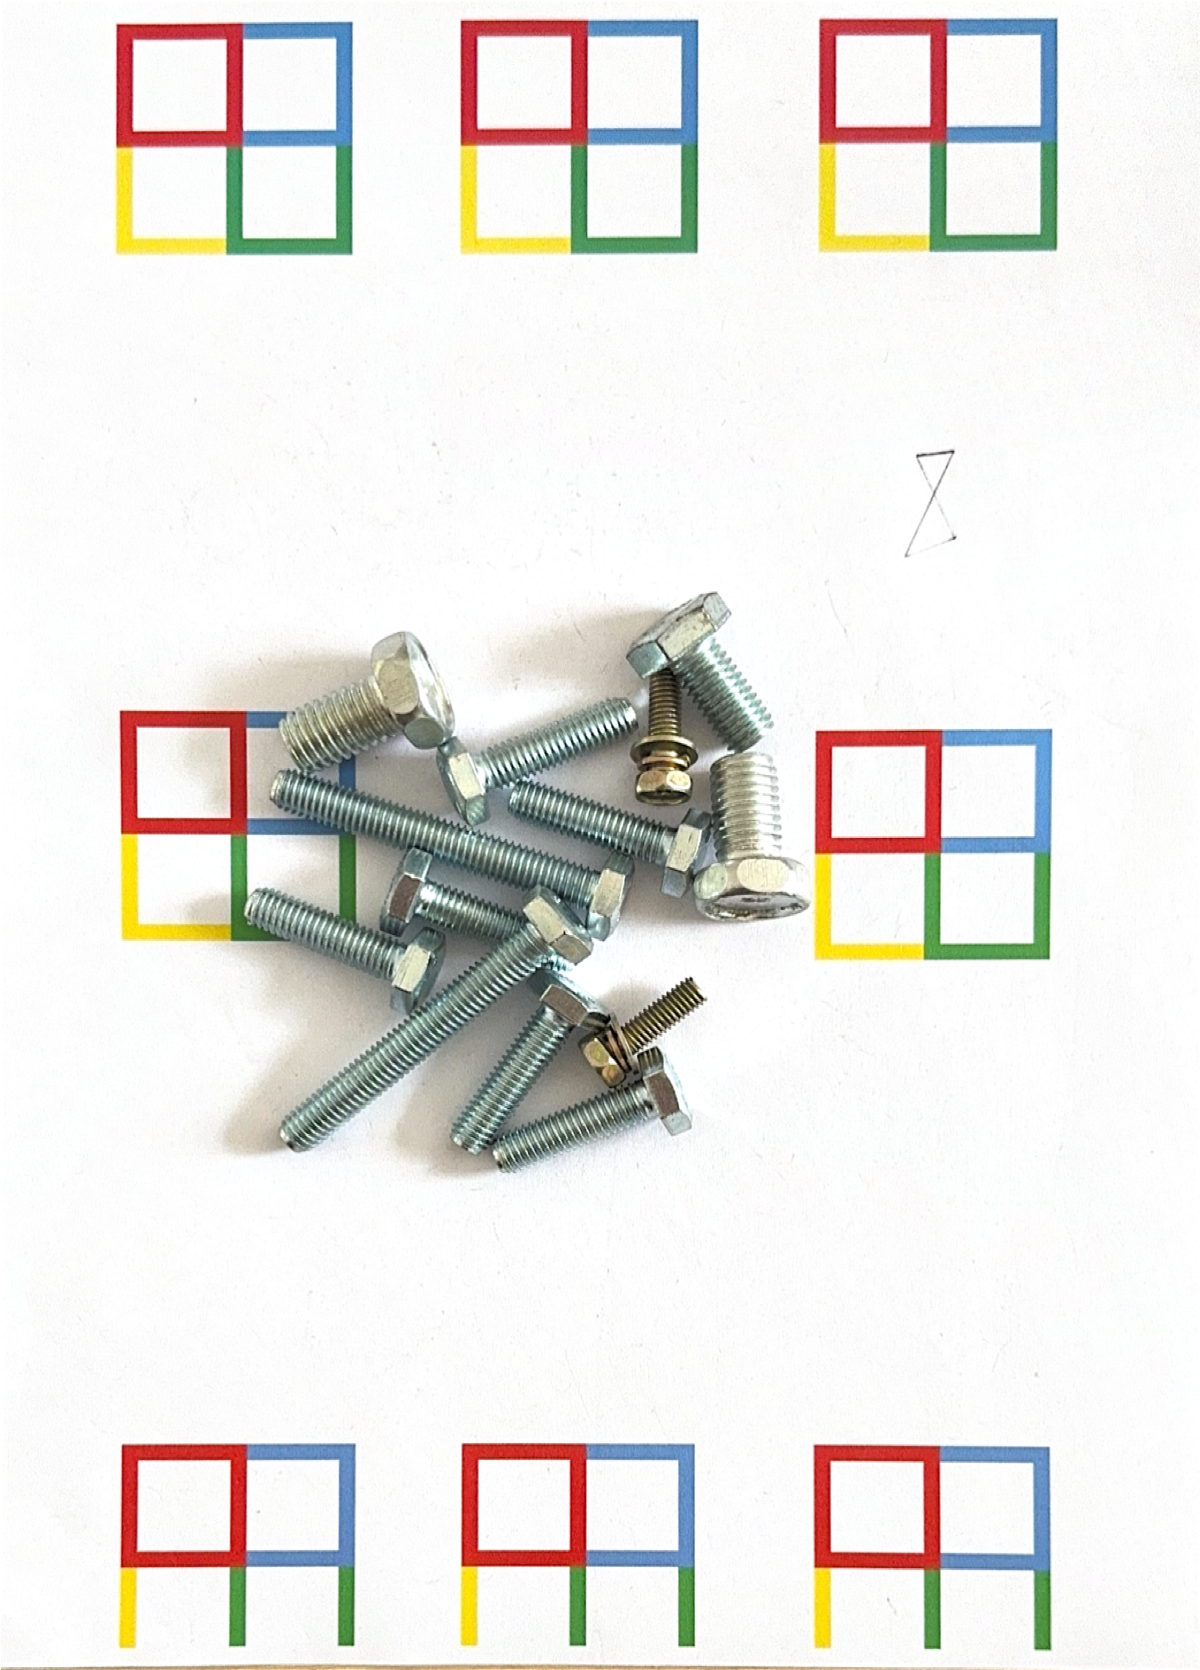
\includegraphics[width=\textwidth]{../data/05.png}
        \caption{05.png 原图}
    \end{subfigure}
    \begin{subfigure}{0.48\textwidth}
        
\includegraphics[width=\textwidth]{../output/05.png}
        \caption{05.png 分割结果 (发生严重粘连)}
    \end{subfigure}
\end{figure}

\section{结果分析}

\subsection{客观评价}
整体而言，本算法在处理散落、未发生严重遮挡的螺丝时表现出色。针对 \texttt{01.png} 至 \texttt{04.png} 图像，Otsu 自适应阈值法能够无视不同图片间的整体亮度差异，准确区分出前景与背景；基于先验特征设计的“面积过滤”与“实心率过滤（Solid Ratio > 0.75）”策略表现出极强的鲁棒性，成功过滤掉了背景杂散点与画面中大量的六角形中空螺母（干扰物），未出现将螺母误判为螺丝的现象，保证了 False Positive 几乎为 0。

\subsection{存在的问题与原因分析}
尽管大部分散落的螺丝分割准确，但在特定的困难场景下，依然存在以下分割缺陷：

\begin{enumerate}
    \item \textbf{严重粘连导致的欠分割（Under-segmentation/Merge）}：
    \begin{itemize}
        \item \textbf{现象}：在测试图 \texttt{05.png} 中，大量螺丝高度重叠堆积在一起。当前基于全局二值化和连通域的算法会将这一整团螺丝识别为同一个单一的连通分量，从而导致严重漏分（Miss），退化成了语义分割而非实例分割。部分图片（如 \texttt{01.png} 等）中若有两个螺丝发生轻微接触，也会被分配成相同的颜色（识别为1个实例）。
        \item \textbf{原因}：传统连通域分析算法不具备高级空间语义理解能力，只要前景像素之间存在 8-邻域或 4-邻域的连通性，就会将其归为同一实例。我也曾尝试利用距离变换（Distance Transform）结合分水岭（Watershed）算法或多次迭代的腐蚀（Erosion）来寻找局部极大值（种子点）拆分实例，但由于螺丝形状细长、不规则，距离变换后极易在一个长条形螺丝内部产生多个断裂的极大值区域，反而会导致单个螺丝被过分割（Over-segmentation）切碎成多段。因此，权衡之下回退至基础连通域分析。
    \end{itemize}
    \item \textbf{局部边缘残缺与内部分割不完整（Incomplete）}：
    \begin{itemize}
        \item \textbf{现象}：仔细观察掩码边缘可以发现，部分螺丝的高亮反光处以及极度凹陷的螺纹阴影处，掩码边界不够平滑，偶尔存在轻微的“咬边”现象；或者螺丝体内部出现极细小的未被标记孔洞。
        \item \textbf{原因}：金属表面存在高光反射（Specular Highlights），这部分区域在灰度图上呈现高亮白色，与浅色背景灰度值相近，在全局 Otsu 二值化时易被误分为背景，造成掩码缺失断裂。此外，在进行形态学开运算时（用于消除噪点），会不可避免地对物体的精细边缘（如锋利的螺纹）造成一定的平滑或侵蚀损伤。
    \end{itemize}
\end{enumerate}

\subsection{总结}
综上所述，传统的基于二值化与形态学过滤的图像处理方法，对于有特定先验形状且独立分布的物体提取效率极高，且解释性强、计算开销小；但在处理物体严重重叠、存在强烈金属反光等复杂场景时，存在不可逾越的局限性。要彻底解决重叠遮挡与高光截断的问题，建议引入基于深度学习的实例分割网络（如 Mask R-CNN 或 YOLOv8-seg），通过数据驱动的方式学习物体更高阶的语义及遮挡边界特征。

\end{document}